%======================================================================
\chapter{Physics at the mesoscale}
\label{ch:swimming at the mesoscale}

\markright{Physics at the mesoscale}
%======================================================================

\section{Low Renolds number regime}
\label{st:lowreynoldsnumber}

At the mesoscale, where objects such as bacteria and colloidal particles operate, the physical world is governed by a regime in which viscous forces dominate over inertial ones. This regime is characterized by a small Reynolds number (Re), a dimensionless quantity that compares inertial to viscous effects. Therefore, the force applied at that moment will describe the movement or displacement performed, not deppending on any past force, this is a characteristic of an overdamped system. In his seminal lecture, Life at Low Reynolds Number, Purcell highlighted the surprising and often counterintuitive behaviors that emerge in such environments~\cite{purcell2014life}. For instance, time-reversible motion — common at macroscopic scales — is ineffective for propulsion at low Re, necessitating non-reciprocal strategies like flagellar rotation or body undulation. This leads to the scallop theorem, that states that an animal with such degrees of freedom — in a viscous regime — will not have a net displacement. 

This whole process can be described by the Navier-Stokes equation without the inertia terms, leaving us without any time deppending terms as shown in Eq. (\ref{eq:Navier-Stokes}). 

\begin{equation}
  - \nabla p + \eta \nabla ^2 \vec{v} = 0
  \label{eq:Navier-Stokes}
\end{equation}

This has been a topic of interest for researchers that are constantly looking for ways of transportation in those environments for specific tasks. Unfortunately this is not the only challenge we face when moving at the microscale.

\section{Brownian Motion and Thermal Fluctuations}
\label{st:brownianmotion}

Even though this is a viscous regime, particles are not static. At small length scales, such as those of colloidal particles or bacteria, random thermal fluctuations become a dominant source of motion. This phenomenon, known as \textit{Brownian motion}, was first explained quantitatively by Albert Einstein in 1905. He demonstrated that the irregular paths observed in microscopic particles suspended in fluid result from collisions with the molecules of the surrounding medium~\cite{einstein1906theory}.

Einstein's work provided one of the first convincing arguments for the molecular nature of matter and led to a mathematical description of how these random movements accumulate over time. Specifically, he derived that the mean squared displacement (MSD) of a particle grows linearly with time:

\begin{equation}
  \langle x^2(t) \rangle = 2Dt\text{,}
  \label{eq:msd}
\end{equation}

where $D$ is the diffusion coefficient, a measure of how quickly particles spread out. Einstein further related this coefficient to measurable physical parameters through the expression:

\begin{equation}
  D = \frac{k_{B}T}{6\pi \eta R}\text{,}
  \label{eq:diffusioncoefficient}
\end{equation}

where $k_B$ is Boltzmann’s constant, $T$ the absolute temperature, $\eta$ the dynamic viscosity of the fluid, and $R$ the radius of the spherical particle. This relation — often referred to as the \textit{Einstein-Stokes equation} — is foundational in soft matter and colloidal physics.

In the systems considered in this thesis, Brownian motion plays a crucial role in the dynamics of passive colloids and must be accounted for even in the presence of external fields or active agents, such as bacteria.

\vspace{1em}

While Einstein’s formulation captures the long-term diffusive behavior of Brownian particles, it does not account for their instantaneous dynamics. To describe how particles move under both viscous damping and random thermal forces, we turn to a stochastic differential equation known as the \textit{Langevin equation}.

\subsection{Stochastic Representation}
\label{stochasticrepresentation}

The Langevin equation \cite{uhlenbeck1930theory} in one dimension, including inertial effects, damping, and thermal noise, can be written as:

\begin{equation}
  m\ddot{x} = F - \lambda \dot{x} + \eta(t)\text{,}
  \label{eq:newton}
\end{equation}

where $m$ is the particle mass, $\lambda$ is the damping coefficient, and $\eta(t)$ is a stochastic force representing thermal noise. For simplicity, we write the velocity as $v = \dot{x}$, leading to:

\begin{equation}
  m\frac{dv}{dt} = F - \lambda v + \eta(t)\text{.}
  \label{eq:newtonv}
\end{equation}

Discretizing time with a small step $dt$, we apply the definition of a derivative:

\begin{equation}
  m \frac{v(t + dt) - v(t)}{dt} = F - \lambda v(t) + \eta(t)\text{.}
  \label{eq:newtonderivative}
\end{equation}

The thermal noise term $\eta(t)$ is modeled as a Gaussian white noise process:

\begin{equation}
  \eta(t)\, dt = g\, dW\text{,}
  \label{eq:eta}
\end{equation}

where $dW$ is a Wiener process (increment of Brownian motion) such that:

\begin{equation}
  \langle dW \rangle = 0\,, \quad \langle dW^2 \rangle = dt\text{.}
  \label{eq:meanvariance}
\end{equation}

Solving for $v(t + dt)$ gives:

\begin{equation}
  v(t + dt) = v(t) + \frac{dt}{m}(F - \lambda v(t)) + g\, dW\text{.}
  \label{eq:velocityplusone}
\end{equation}

Now, assuming no deterministic force ($F = 0$) — as is the case for free passive particles:

\begin{equation}
  v(t + dt) = v(t) - \frac{\lambda dt}{m} v(t) + g\, dW\text{.}
  \label{eq:noforce}
\end{equation}

Taking the expectation value (mean) of both sides:

\begin{equation}
  \langle v(t + dt) \rangle = \langle v(t) \rangle - \frac{\lambda dt}{m} \langle v(t) \rangle + g \langle dW \rangle\text{.}
  \label{eq:mean}
\end{equation}

Since $\langle dW \rangle = 0$, the last term vanishes:

\begin{equation}
  \langle v(t + dt) \rangle = \langle v(t) \rangle \left( 1 - \frac{\lambda dt}{m} \right)\text{.}
\end{equation}

In the limit of small $dt$, this leads to the differential equation:

\begin{equation}
  \frac{d}{dt} \langle v(t) \rangle = - \frac{\lambda}{m} \langle v(t) \rangle\text{,}
  \label{eq:derivative}
\end{equation}

whose solution is:

\begin{equation}
  \langle v(t) \rangle = \langle v(0) \rangle\, e^{-\lambda t / m}\text{.}
\end{equation}

This result shows that the average velocity of a particle in a viscous fluid decays exponentially due to damping. The characteristic timescale $\tau = m/\lambda$ describes how quickly the particle forgets its initial velocity, after which the motion becomes diffusive.

%%%%

\subsection{Velocity Statistics and Energy Equipartition}

To compute the variance of the velocity, we start again from the Langevin equation in discretized form, without external forces:

\begin{equation}
  v(t + dt) = v(t) - \frac{\lambda}{m} v(t) dt + \frac{g}{m} dW \text{.}
\end{equation}

Squaring both sides:

\begin{align}
  v(t + dt)^2 &= \left[ v(t) - \frac{\lambda}{m} v(t) dt + \frac{g}{m} dW \right]^2 \text{,}\\
              &= v(t)^2 + \left( \frac{\lambda}{m} \right)^2 v(t)^2 dt^2 + \left( \frac{g}{m} \right)^2 dW^2 \nonumber \\
              &\quad - 2 \frac{\lambda}{m} v(t)^2 dt + 2 \frac{g}{m} v(t) dW - 2 \frac{\lambda g}{m^2} v(t) dW \text{.}
\end{align}

Now we take the expectation value:

\begin{align}
  \langle v(t + dt)^2 \rangle &= \langle v(t)^2 \rangle + \left( \frac{\lambda}{m} \right)^2 \langle v(t)^2 \rangle dt^2 + \left( \frac{g}{m} \right)^2 \langle dW^2 \rangle \nonumber \\
                              &\quad - 2 \frac{\lambda}{m} \langle v(t)^2 \rangle dt + 2 \frac{g}{m} \langle v(t) \rangle \langle dW \rangle - 2 \frac{\lambda g}{m^2} \langle v(t) \rangle \langle dW \rangle \text{.}
\end{align}

Using the properties of the Wiener process:

\[
  \langle dW \rangle = 0, \quad \langle dW^2 \rangle = dt \text{.}
\]

And neglecting second-order small terms (\( dt^2 \)), we obtain:

\begin{equation}
  \langle v(t + dt)^2 \rangle = \langle v(t)^2 \rangle + \frac{g^2}{m^2} dt - 2 \frac{\lambda}{m} \langle v(t)^2 \rangle dt \text{.}
\end{equation}

Taking the continuous limit:

\begin{equation}
  \frac{d}{dt} \langle v(t)^2 \rangle = -2 \frac{\lambda}{m} \langle v(t)^2 \rangle + \frac{g^2}{m^2} \text{.}
\end{equation}

This is a linear first-order ODE. Solving it with variation of constants yields:

\begin{equation}
  \langle v(t)^2 \rangle = \frac{g^2}{2 \lambda m} + D e^{-2 \lambda t / m} \text{.}
\end{equation}

As \( t \to \infty \), the exponential term vanishes and we get the stationary value:

\begin{equation}
  \langle v(\infty)^2 \rangle = \frac{g^2}{2 \lambda m} \text{.}
\end{equation}

From the equipartition theorem, we know that the average kinetic energy is:

\[
  \frac{1}{2} m \langle v^2 \rangle = \frac{1}{2} k_B T \text{.}
\]

Therefore:

\begin{equation}
  \langle v^2 \rangle = \frac{k_B T}{m} \text{.}
\end{equation}

Matching this to our stochastic result:

\begin{equation}
  \frac{k_B T}{m} = \frac{g^2}{2 \lambda m} \quad \Rightarrow \quad g^2 = 2 \lambda k_B T, \quad g = \sqrt{2 \lambda k_B T} \text{.}
\end{equation}

This defines the noise amplitude in terms of temperature, viscosity, and Boltzmann’s constant.

\subsection{Overdamped Dynamics and Diffussion}

In the overdamped limit, inertia is negligible, so the Langevin equation becomes:

\begin{equation}
  0 = F - \lambda \frac{dx}{dt} + \eta(t) \text{.}
\end{equation}

Solving for the velocity:

\begin{equation}
  \frac{dx}{dt} = \frac{1}{\lambda} (F + \eta(t)) \text{.}
\end{equation}

For free diffusion (\( F = 0 \)):

\begin{equation}
  \frac{dx}{dt} = \frac{1}{\lambda} \eta(t) \text{.}
\end{equation}

Using stochastic calculus with \( \eta(t) dt = g dW \), we write:

\begin{equation}
  x(t + dt) = x(t) + \frac{g}{\lambda} dW \text{.}
\end{equation}

\paragraph{Mean Position}

Taking the expectation:

\begin{equation}
  \langle x(t + dt) \rangle = \langle x(t) \rangle + \frac{g}{\lambda} \langle dW \rangle = \langle x(t) \rangle \text{.}
\end{equation}

So the mean position remains constant in free diffusion.

\paragraph{Mean Square Displacement (MSD)}

Squaring the position update:

\begin{equation}
  x(t + dt)^2 = x(t)^2 + 2 \frac{g}{\lambda} x(t) dW + \left( \frac{g}{\lambda} \right)^2 dW^2 \text{.}
\end{equation}

Taking the expectation:

\begin{align}
  \langle x(t + dt)^2 \rangle &= \langle x(t)^2 \rangle + 2 \frac{g}{\lambda} \langle x(t) \rangle \langle dW \rangle + \frac{g^2}{\lambda^2} \langle dW^2 \rangle \text{,}\\
  &= \langle x(t)^2 \rangle + \frac{g^2}{\lambda^2} dt \text{.}
\end{align}

In differential form:

\begin{equation}
  \frac{d}{dt} \langle x(t)^2 \rangle = \frac{g^2}{\lambda^2} \text{.}
\end{equation}

Using \( g^2 = 2 \lambda k_B T \), we substitute:

\begin{equation}
  \frac{d}{dt} \langle x(t)^2 \rangle = \frac{2 k_B T}{\lambda} \text{.}
\end{equation}

Integrating gives the mean squared displacement (MSD):

\begin{equation}
  \langle x(t)^2 \rangle = \frac{2 k_B T}{\lambda} t \text{.}
\end{equation}

This is the classical diffusion result, where the diffusion coefficient is \( D = \frac{k_B T}{\lambda} \), consistent with Einstein's expression.



%%%%
%This raises a fundamental question: Can these fluctuations be harnessed to perform useful work? This idea lies at the heart of thought experiments such as the Feynman ratchet, which challenge our understanding of thermodynamics at microscopic scales.


\begin{figure}[H]
  \begin{center}
    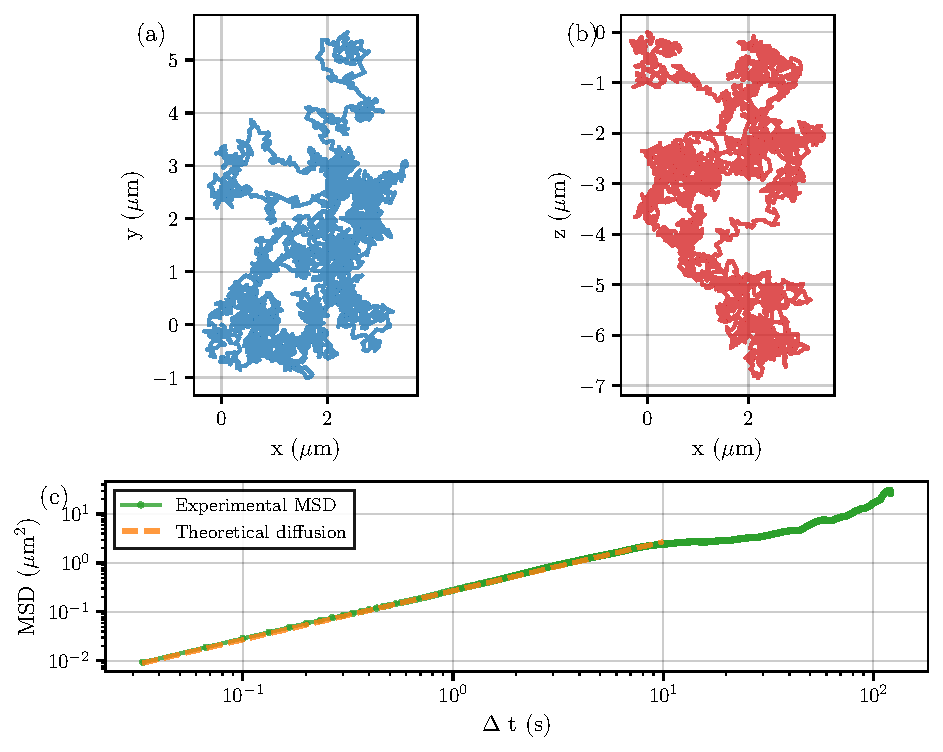
\includegraphics[width=0.8\textwidth]{figures/passivebrowniantrajectory.pdf}
  \end{center}
  \caption[Example of brownian motion]{A colloidal particle undergoes random, thermally induced displacements in a fluid medium. \textbf{Panel a)} shows the trajectory of the particle. \textbf{ Panel b)} shows the corresponding mean squared displacement (MSD) as a function of time, illustrating the linear relationship predicted by Einstein for diffusive behavior (orange) and the one obtained through a numerical simulation (blue).}\label{fig:passivebrowniantrajectory}
\end{figure}


